% !TEX root = ./thesis.tex

\chapter{Introduction}
\label{ch:intro}

% Outline:
% - successes of Neural network models
% - specifically for spacial related field (spatial transformer network, video thing)
% - VizDoom and
% - we propose
% - potential usages of the proposed system: SLAM, loop closure detection
% - analyses description
%
% Space-time video completion \cite{Wexler2004}
% % Deep learning for visual understanding: A review \cite{Guo2016}
%
% Loop closure detection for visual SLAM systems using deep neural networks \cite{Gao2015}
% Authors build a denoising autoencoder with sparse objective adding continuity objective.
% Continuity objective enforces L2 similarity between extracted features for consecutive frames. They use dataset: freiburg2 slam.
%
% Loop Closure Detection for Visual SLAM Using PCANet Features.
% Unsupervised learning to detect loops using deep neural networks for visual SLAM system.
% VLAD-Based Loop Closure Detection For Monocular SLAM \cite{Xia2016, Gao2015a, Huang2016}

Localization tasks represent a significant challenge in artificial intelligence (AI).
In particular, localization is extremely important to such AI areas as robotics, self-driving vehicles, and micro-surgery, to name a few \cite{Wang2017, Mountney2006}.
Such tasks as simultaneous localization and mapping (SLAM) \cite{Cadena2015, Zikos2016}, loop closure detection \cite{Xia2016, Gao2015a, Huang2016}, and correspondence learning \cite{Boscaini2016} try to solve some form of localization problem.

We can generally define localization as a task of extracting, tracking or predicting object's position in some environment from available sensory data. As, for example, for self-driving vehicles it might be important to track and predict relative position of the pedestrians within the field of view from visual data \cite{Dollar2009}. The same kind of data can be used to extract positions and dimensions of the objects, manipulated by automated-robots \cite{Hernandez2016}. Visual data comes in form of sequences of discretized images containing 3 color channels (RGB) and often additional channel with depth information (RGBD) \cite{Long2015}. Models like that are typically trained with annotated data.

In this work we are going to focus on unsupervised localization in artificial environments such as computer games. Recent successes in reinforcement learning \cite{Silver, Lample2016} has proven, that, given access to computational resources and sufficient amounts of training data, even ill-defined machine-learning problems can be solved with high quality (comparable to human) results. In this work we would like to take advantage of the data-generation techniques, created for reinforcement learning \cite{Brockman2016, Kempka2016}, in order to solve localization problem in an unsupervised manner. More specifically, we are going to use the 3D engine of a first-person shooter (FPS) computer game \texttt{Doom II} in order to generate sufficient amount visual data for training.

We propose a model that extracts positional information of the player from the current view.
Visual data is typically high dimensional and each image might contain tens of thousands of features. Meanwhile, we know, that current view can be compactly and unambiguously described by the current position of the player and the direction of the view. Therefore, we can use the position and the direction of the view as low-dimensional latent representation of high-dimensional visual data. Furthermore, continuous nature of these latent features allows us to state, that there exists a low-dimensional manifold, on which all player's movements maintain the continuous nature. We, therefore, try to build a deep-learning model for extracting such a manifold from the visual data.

\begin{figure}[t!]
	\centering
	\subfigure[Example video data, recorded from the first person view of a player in the shooter game  \texttt{Doom II}.]{
  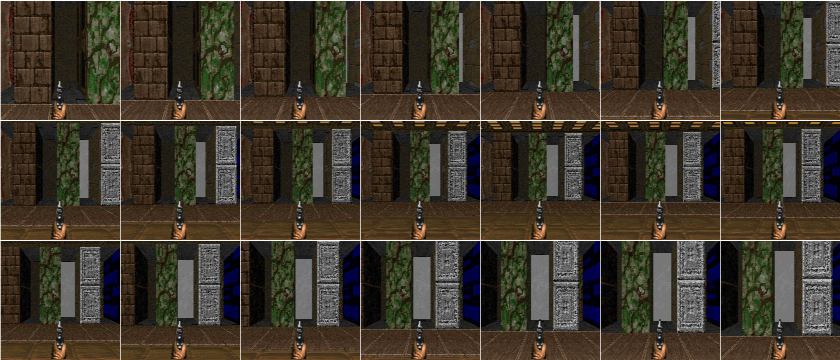
\includegraphics[width=.99\textwidth]{sprite2_2.png}
	}\\
	\subfigure[Example 3-dimensional embedding produced by the model.]{
    	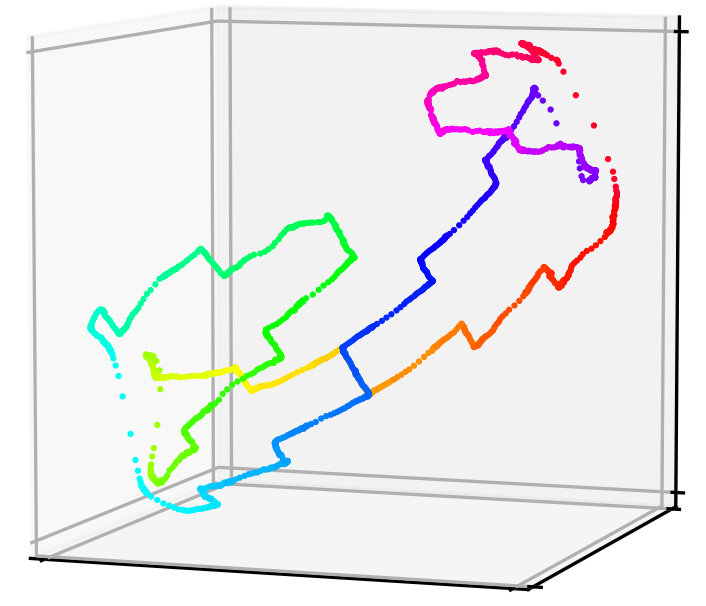
\includegraphics[width=.45\textwidth]{cmp2/cnn_3.png}
	}
	\subfigure[Visualization of the actual player's path.]{
    
\includegraphics[width=.45\textwidth]{path.png}
	}
    	\caption{Visualization of spatial information extraction from video signal by an unsupervised autoencoder based model. The model takes a sequence of RGBD images as input (top), observed by the actor while walking along some path. Model projects each frame into a lower dimensional space in order to extract information, relevant to the position of the player (bottom left). Sequential frames are displayed in similar colors. Bottom-left picture schematically draws the actual trajectory of the player.}
    	\label{fig:intro_ex}
\end{figure}

We propose a deep learning technique, that learns a mapping of unlabeled high-dimensional visual data in RGBD format into a continuous low-dimensional latent feature space (see figure \ref{fig:intro_ex}(a)). We describe a training method, that allows robust learning of such a mapping even for extremely high compression ratios of 10000:1, although with unavoidable information loss. Furthermore, we describe a set of regularization techniques, allowing to reveal latent spatial relations in the input data and, at least for inputs of moderate complexity, build approximate predictions in the latent feature space.

Several models have been successfully applied to unlabeled data allowing to construct a dense manifold representation of some visual concepts \cite{Li2015, Kingma2013, Goodfellow2014}.
While these techniques succeeded in encoding data in a lower dimensional space of independent features, they make no assumption about the nature of these features.
We expect, that extremely low-dimensional representation of the spatially related data  would be tightly coupled with that spatial information.
To enforce this expectation we apply additional constraints to the model to preserve geometrical qualities in the latent features.
Existing research on extracting interpretable features suggest, that such extraction is possible, although might significantly complicate the training process \cite{Lei2016, Kulkarni2015}.

An ultimate goal of this project can be viewed as a direct and inverse graphics engine in form of an autoencoder. In such model encoder network performs the mapping of current visual information into the coordinate space; decoder learns to reconstruct the image from the positional information.
The goal can be described as achieving an autoencoder objective in form of perfect image reconstruction, while producing a dense continuous spatial manifold in the latent feature space.
Successfully achieving this goal, we will be able to produce the player's view given the position and vise-versa: determine possible position of the player by the current view.
This model can behave as an ultimate solution for SLAM, correspondence and loop detection problems.
We understand, that that goal is unlikely to be fully achieved, given limited computational resources, discrete nature of actual training data and often non-static characteristics of real-world environments.

Later chapters are organized as follows.
We continue the current discussion in chapter \ref{ch:rewo} by describing recent research advances, relevant to the task at hand.
In chapter \ref{ch:tede} we provide technical details about artificial neural network, their training techniques, and common complications of the training process.
Chapter \ref{ch:mode} describes our learning method and additional model constraints along with underlying motivation.
Finally, in chapter \ref{ch:eval} we explore the advantages of our method when applied to actual data.
Chapter \ref{ch:conc} concludes the results of our research and outlines possible future work.
